\myparagraph{Purpose}
The main feature of \textit{AutomatedSOS} is to check the health status of the user and to detect any critical situation.
The detection of critical situation computes a huge number of data, which provides several information about the health status of the user, so \textit{AutomatedSOS} provides also a service to show the health status of the user.

\myparagraph{Scenario}
Silvia is worried about her grandmother's health status because she is been tired for a few days. Two month ago Silvia installed on her grandmother phone \textit{AutomatedSOS} application.
In order to calm herself, Silvia takes the phone of her grandmother, opens \textit{AutomatedSOS} and logs in.
In the main page of the application there is the summary of the health status and everything looks ok.
To avoid any doubt Silvia clicks on the "\textit{Details}" button and checks all the statistics about last week and last month value of pressure and heartbeat.

\myparagraph{Use Case}
The \textit{Health Status Visualization} use case is analyzed in Table \ref{table:healthStatus}.

\myparagraph{Activity Diagram}
The \textit{Healt Status Visualization} activity diagram is shown in Figure \ref{img:healthStatusActivityDiagram}.

\myparagraph{Mockup}
The \textit{Healt Status Visualization} mockup is shown in Figure \ref{img:healthStatusMockup}.

\myparagraph{Functional requirements}
\begin{enumerate}
  \item The system must let the user view his personal health status at anytime;
  \item The system must update the health status of the user at anytime it receives new data from the devices;
  \item The system must stores the data in order to provide monthly and weekly statistics.
\end{enumerate}

\begin{center}
\begin{table}[H]
\begin{tabular}{ | l | p{0.75\linewidth} | }
  \hline
    Actor & \textbf{User} \\ \hline
    Goal & \textbf{[G.7]} \\ \hline
    Input Condition & A \textbf{User} wants to view his/her health status.\\ \hline
    Event Flow & \begin{minipage}[t]{0.7\textwidth}
      \begin{enumerate}
        \item The \textbf{User} opens \textit{AutomatedSOS} application;
        \item The \textbf{User} logs in;
        \item The \textbf{User} clicks on the "\textit{Health Status}" button;
        \item The system shows to the \textbf{User} the data acquired on him/her with the relative computation of the health status.
      \end{enumerate}
    \smallskip
  \end{minipage} \\ \hline
  Output Condition & The \textbf{User} views his/her personal health status monitored by \textit{AutomatedSOS}\\ \hline
  Exceptions & If the system does not acquire enough data to produce statistics it notifies the \textbf{User} with a warning.  \\ \hline
\end{tabular}
\caption{\textit{Health Status Visualization} use case}
\label{table:healthStatus}
\end{table}
\end{center}

\begin{figure}[H]
\begin{center}
  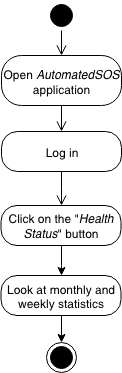
\includegraphics{img/activity/HealthStatus.png}
  \hspace{0.05\linewidth}
  \centering
  \caption{\textit{Health Status Visualization} activity diagram from user's point of view}
  \label{img:healthStatusActivityDiagram}
\end{center}
\end{figure}

\begin{figure}[H]
\begin{center}
  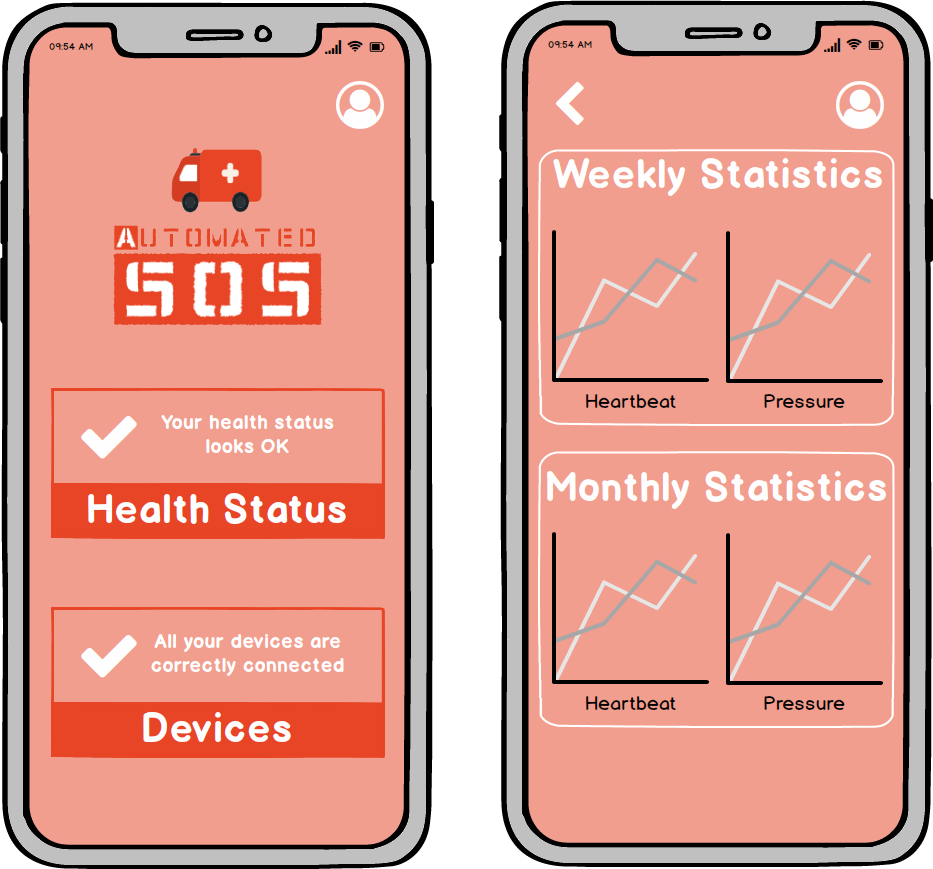
\includegraphics[width=\textwidth]{img/mockup/Health_Status.png}
  \hspace{0.05\linewidth}
  \centering
  \caption{\textit{Health Status Visualization} mockup}
  \label{img:healthStatusMockup}
\end{center}
\end{figure}
